%!TEX root = ../../Heun_Dale_Haney_A_dynamic_approach_to_input_output_modeling.tex
%%%%%%%%%%%%%%%%%%%%% chapter.tex %%%%%%%%%%%%%%%%%%%%%%%%%%%%%%%%%
%
% sample chapter
%
% Use this file as a template for your own input.
%
%%%%%%%%%%%%%%%%%%%%%%%% Springer-Verlag %%%%%%%%%%%%%%%%%%%%%%%%%%
%\motto{Use the template \emph{chapter.tex} to style the various elements of your chapter content.}
\motto{Where there is no reliable accounting 
and therefore no competent knowledge 
of the economic and ecological effects of our lives, 
we cannot live lives that are economically and ecologically responsible. 
It is futile to plead and protest and lobby 
in favor of public ecological responsibility while, 
in virtually every act of our private lives, 
we endorse and support an economic system that is by intention, 
and perhaps by necessity, 
ecologically irresponsible.~\emph{\cite[p.~26]{Berry1998}}

\hfill---\emph{Wendell Berry}}


%%%%%%%%%%%%%%%%%%%%%%%%%%%%%%%%%%
%%%%%%%%%% Introduction %%%%%%%%%%
%%%%%%%%%%%%%%%%%%%%%%%%%%%%%%%%%%
\chapter{Introduction: The end of an era}
% Always give a unique label
\label{chap:intro}
% use \chaptermark{}
% to alter or adjust the chapter heading in the running head
\chaptermark{Introduction}
%%%%%%%%%%%%%%%%%%%%%%%%%%%%%%%%%%
%%%%%%%%%%%%%%%%%%%%%%%%%%%%%%%%%%
%%%%%%%%%%%%%%%%%%%%%%%%%%%%%%%%%%


%% \abstract{Each chapter should be preceded by an abstract (10--15 lines long) that summarizes the content. The abstract will appear \textit{online} at \url{www.SpringerLink.com} and be available with unrestricted access. This allows unregistered users to read the abstract as a teaser for the complete chapter. As a general rule the abstracts will not appear in the printed version of your book unless it is the style of your particular book or that of the series to which your book belongs.\newline\indent
%% Please use the 'starred' version of the new Springer \texttt{abstract} command for typesetting the text of the online abstracts (cf. source file of this chapter template \texttt{abstract}) and include them with the source files of your manuscript. Use the plain \texttt{abstract} command if the abstract is also to appear in the printed version of the book.}

%% Use the template \emph{chapter.tex} together with the Springer document class SVMono (monograph-type books) or SVMult (edited books) to style the various elements of your chapter content in the Springer layout.

\abstract*{**** Re-write the abstract. ****
In this chapter we give our motivation for writing this book. 
We outline some of the models and subsequent metaphors 
that have been used to describe the economy---clockwork, 
machine, engine---and suggest a new metaphor---the 
metabolism of an organism.
We give an overview of Leontief Input-Output methods
and their extension to include energy and material inputs
and waste flows out of the economy.
We then propose a new Input-Output analysis method,
fitting to the new metaphor of the metabolic economy;
a dynamic accounting framework that includes accumulation of stocks
within economic sectors.}


The world is entering a new economic era. 
There is widespread agreement that economic growth in mature economies 
is unlikely reach the rates seen in the 20$^\mathrm{th}$~Century ever again.  
Indeed, over the last fifty years, 
the economic growth rate of the 
Organisation for Economic Co-operation and Development (OECD) 
member states has fallen precipitously. 
The long-term forecast from the OECD is that mature economies 
will grow only 1.5--2.0\% annually over the next fifty years. 
Similarly, the US Congressional Budget Office forecasts 
an average growth rate of 2.2\% for the US economy 
from 2018--2024.\cite{OECD2014,CBO2014}

The stagnation of economic growth for mature economies 
(as measured by annual percentage change in GDP per capita) 
is even more striking 
when compared to the explosive growth in emerging economies. 
Figure~\ref{fig:gdppc} shows the 5-year trailing average 
of economic growth rates for the China, India, and the OECD since 1965. 
The trendline of the OECD is clearly downward, 
while the trendline of Chinese and Indian growth is clearly upward.  
Indeed, the OECD itself says that the 
``combined GDP of China and India was 33\% of the OECD in 2010 
(on a PPP basis), 
but is expected to rise to 73\% by 2060.''~\cite[p. 214]{OECD2014} 
Slowing OECD growth illustrates that mature economies are hitting a wall.

\begin{figure}
\centering\
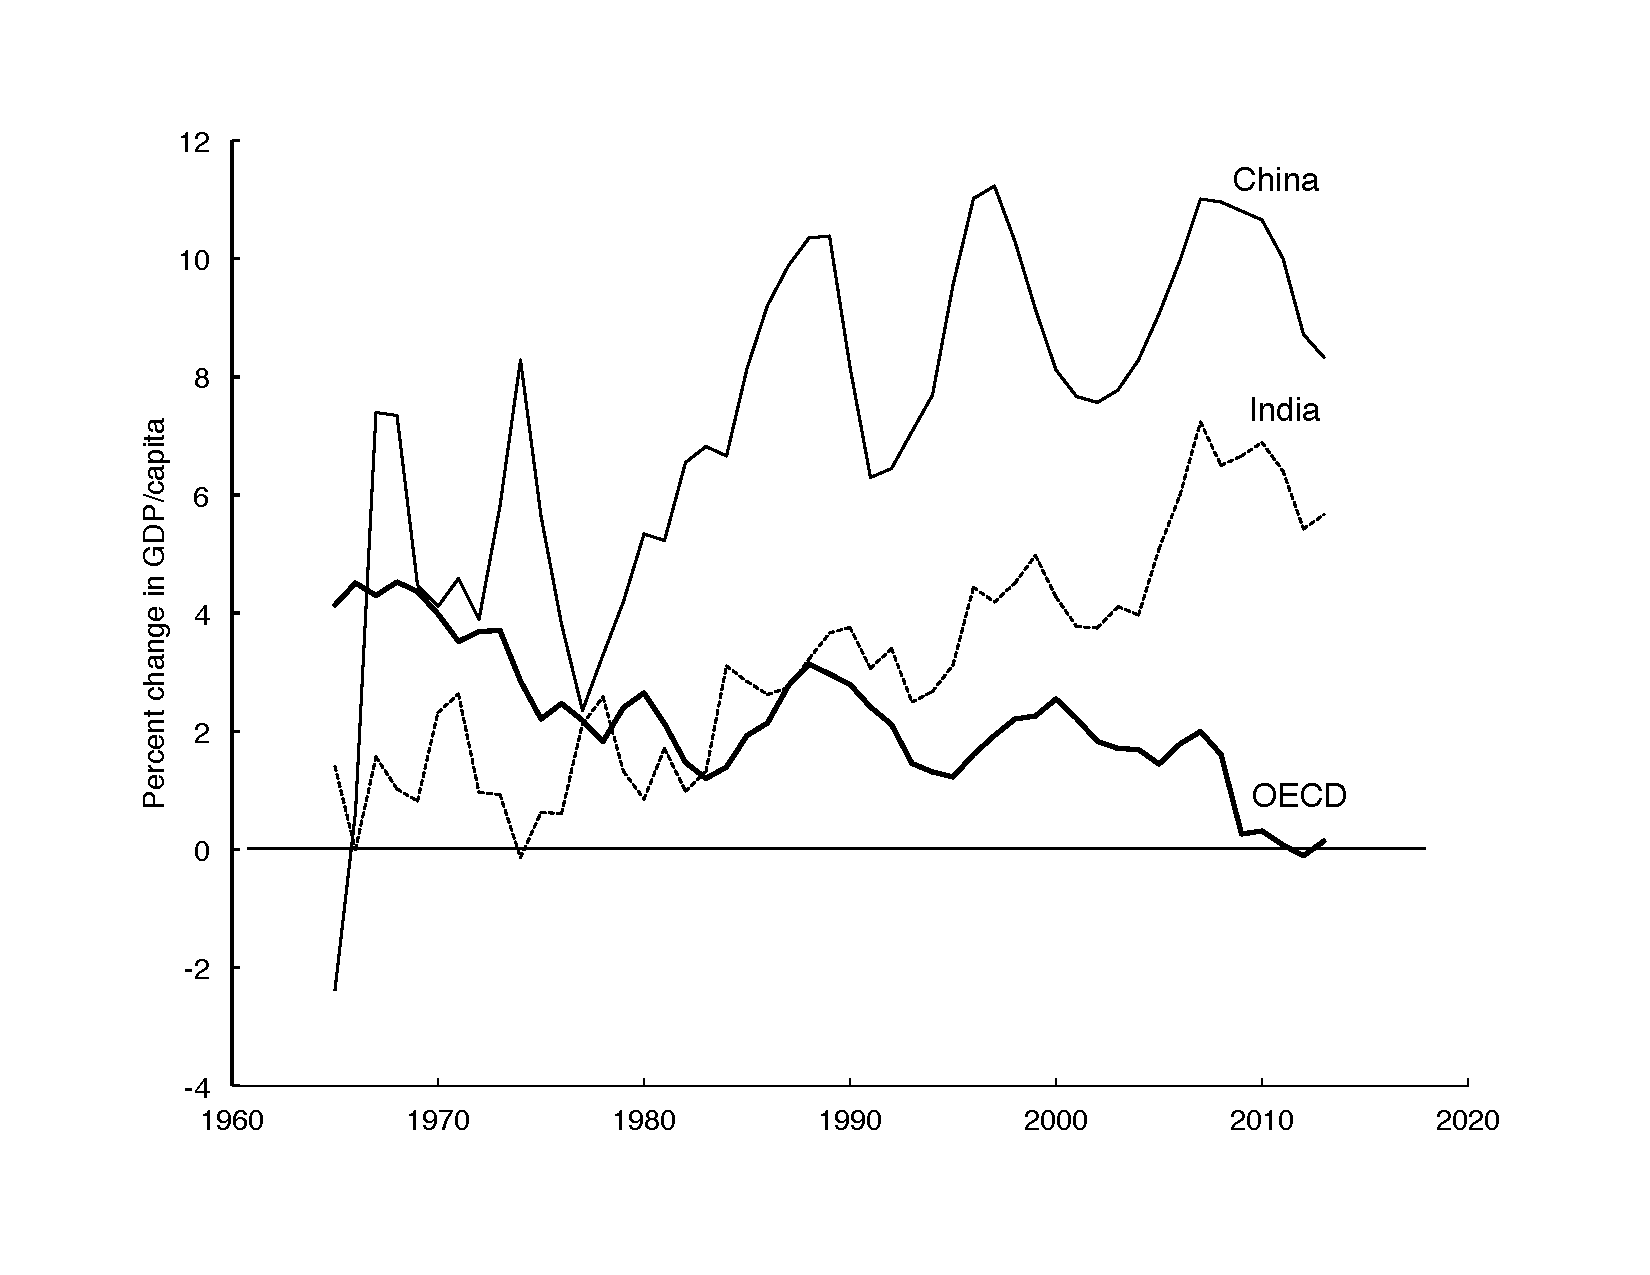
\includegraphics[width=\linewidth]{Part_0/Chapter_Introduction/images/EconGrowth.pdf}
\caption[Economic growth, 1960--2013]{Five-year trailing averages of economic growth, 
1965--2013.\cite{WorldBank2014}}
\label{fig:gdppc}
\end{figure}

Is stalled economic growth a problem? 
Most analysts believe it is. 
History suggests that growth of GDP 
raises living standards and human well-being,
as measured by various indices. 
Julian Simon's volume, \emph{The State of Humanity}, 
catalogues the great improvements in 
life span, 
housing, 
environment, 
food quality and availability, 
water cleanliness, 
etc.\ 
that have coincided with 
economic growth over the last three centuries.\cite{simon1996} 

Thus, stalled economic growth can be expected 
to be accompanied by slowing or reversing
of the upward trend in quality of living. 
The economic establishment's prescription
to avoid backsliding of quality of life and human well-being
is continued economic growth by (nearly) any means necessary. 
At the moment, continued economic growth appears to be the only 
politically-viable policy instrument.

What do economists believe is causing the slowdown
of economic growth in mature economies? 

Mainstream economic theory considers 
economic growth to be driven by four factors: 
(1) increasing labor utilization as a result of increasing the number of workers or worker hours, 
(2) increasing human capital through improved education levels, skill levels, or health, 
(3) increasing capital/labor ratio because of expanded capital investments, and 
(4) increasing worker productivity due to technological innovation. 
In recent years, the economy has deteriorated on all four factors.
Economist Tyler Cowen argues that large productivity gains 
through innovation have permanently plateaued 
leading to a ``great stagnation'' in economic growth.\cite{Cowen2011}
The Cato Institute's economic growth specialist, Brink Lindsey, 
suggests that growth has permanently stalled, 
because \emph{all four} of the primary drivers of economic growth have plateaued; 
hours worked, 
worker skill level, and
the amount of capital invested per worker 
have reached 
a low, slow, steady state 
and are unlikely to rebound.\cite{lindsey2013} 

The Cowen and Lindsey analyses represent mainstream explanations for the growth slowdown,
and they are based squarely on the assumption that technology augments 
capital and labor, the inputs to economic growth.%
	\footnote{
	The mainstream model for economic growth is encapsulated in the
	Cobb-Douglas production function, which takes the mathematical form
	%
	\begin{equation*}
		y = A k^{\alpha} l^{1-\alpha}
	\end{equation*}	 
	%
	where 
	$y$ is economic output, 
	$A$ is technological progress,
	$k$ is capital stock, 
	$l$ is labor, 
	$\alpha$ is the factor share of capital, and
	$1-\alpha$ is the factor share for labor.
	}
If economic slowdown is caused by anything besides
technology, capital, or labor,
mainstream economic analysis can't provide any assistance
in either diagnosing the problem or prescribing a cure.

We believe that the mainstream approach is too narrow and
that there may be other factors that cause economic slowdown.
In particular,  
we contend that binding constraints on economic growth may arise from
at least two sources: 
material inputs from the biosphere and 
the energy to run the ``economic engine.''

Our approach may be outside the economic mainstream,
but we are not alone. 
There are several inter-disciplinary fields 
(industrial ecology, ecological economics, biophysical economics, and
materials flow analysis)
where the relationship between the 
economy and the biosphere is a natural feature of the intellectual landscape
and assessment of patterns of economic growth and economic downturns  
includes consideration of biophysical limits. 
This emerging paradigm is taking shape with the leadership of theorists
such as 
Robert Ayres~\cite{Ayres:2010ug}, 
Kenneth Boulding~\cite{Boulding1966}, 
Roger Boyd~\cite{boyd2013energy},
Robert Costanza~\cite{Cleveland:1984aa}, 
Herman Daly~\cite{Daly1977}, 
Blair Fix~\cite{Fix:2014aa},
Charles Hall~\cite{hall2011energy}, 
Steven Kopits~\cite{Kopits:2009aa},
Marina Fischer-Kowalski~\cite{F-K1999},
and others.
Throughout this book, we'll refer to this approach as a ``biophysical'' approach
to the economy.

Historically, the biophysical approach led to the insight 
that material and energy constraints could lead to the 
end of the era of economic growth based solely on increased
consumption.
A striking example comes from 
inter-disciplinarian Robert Ayers who, in 1996, presciently described 
how it would end in a financial collapse similar to the ``Great Recession:''

% A striking aspect of mainstream economic analyses is that
% nowhere in the diagnosis of the problem of stalled growth
% does the economy's reliance on the biosphere play a role.
% There is no recognition that the biosphere may place physical limits
% on the economy.
% Because the biosphere places physical limits
% on the economy in terms of
% (1) material inputs and
% (2) the energy to run the economic engine,
% these two binding constraints on economic growth
% should be a part of models of economic growth.

% Yet, mainstream economic growth models
% and the policy prescriptions that emerge from them
% do not identify biophysical limits to the economy
% as a potential a contributor to the economic downturn.
% The above analyses from
% Cowen\cite{Cowen2011} and Lindsey \cite{lindsey2013}
% represent the mainstream explanations for the growth slowdown.
% The analysis relies squarely on a Cobb-Douglas production function
% version of the economy.
% An economy takes inputs of
% labor and capital,
% makes them as  efficient as possible,
% and produces as much as possible.
% Thus, the policy prescriptions based on this model all attempt to
% remedy a broken piece of the production model.
% But, what if the underlying problem is
% reaching biophysical limits to economic scale?
% The mechanical Cobb-Douglas production function model of an economy
% does not work in this situation.
% And the mainstream economic policy prescriptions based on it and that rely
% on an ever growing economy to succeed are off target.
%
% Beyond the economic mainstream lies the next approach.
% Where the relationship between the economy and the biosphere
% is a natural feature of the intellectual landscape
% and patterns of economic growth and economic downturns
% include consideration of biophysical limits.
% This new paradigm is visible in inter-disciplinary fields
% such as industrial ecology and ecological economics.
% However, the new paradigm is still emerging and taking shape,
% led by rigorous theorists such as
% Kenneth Boulding,
% Herman Daly,
% Robert Costanza,
% Charles Hall,
% Robert Ayres
% and many others. [others?]
% They all have one thing in common, they see the end of an era.
% In the mid-1990s,
% inter-disciplinarian Robert Ayers presciently described what the end of the current era,
% which does not reckon with biophysical limits,
% looks like:

\begin{quote}
	It is difficult to say when, or how, the current economic growth ``system'' will collapse;
	it has proved more resilient than many would have predicted. 
	But, unless job-creating growth can be sharply accelerated 
	the choice facing governments is stark: 
	either there will be very sharp and painful cuts 
	in entitlements and social welfare or there will be a financial crisis,
	probably sudden (like the onset of the Great Depression) and probably within twenty years. 
	The traditional Keynesian job creation mechanisms are ineffective or inapplicable, 
	while trade liberalization and ``globalization'' 
	are making the unemployment problem worse, not better.
	Western democracies are, 
	like the passengers on the Titanic, 
	heading ``full steam ahead'' into
	extremely dangerous waters. 
	Icy reality lies dead ahead, 
	already dimly visible through the fog.
	Collision is inevitable, 
	unless we change course sharply.\cite{Ayres:1996aa}
\end{quote}

% We agree with Ayres that the mainstream will soon be forced to come to grips with
% the interconnections between
% the economy and the biosphere.
% Once it does, Ayres suggests that the future health of the economy will depend upon
% its ability to restructure around renewable energy,
% closed material cycles,
% and shifting from goods manufacturing to service provision.

% The ability of society to continue its current pattern
% of analysis and policy prescription, that is,
% to rely on the mainstream Cobb-Douglas production function model of the economy,
% will soon come to an end,
% forcing mature economies reckon with the interconnections between
% the economy and the biosphere.
% With this relationship made explicit,
% he concludes that the future health of an economy depends on
% its ability to restructure around renewable energy,
% closed material cycles,
% and shifting from goods manufacturing to service provision.


%%%%%%%%%% Measuring the wealth of nations %%%%%%%%%%
\section{(Mis)measuring the wealth of nations}
\label{sec:wealth_nations}
%%%%%%%%%%

An ironic consequence of re-connecting economic analysis to the biosphere is a 
re-emergence of the discussion about a nation's wealth. 
Today's mainstream quantification of economic health, GDP, 
measures only \emph{income}, a \emph{flow} of money (currrency) in units 
of, say, \$/year.  
To understand how GDP relates to \emph{wealth} and mis-measures economic health, 
we need to discuss \emph{capital}.

A nation's wealth consists of physical \emph{stock},  
including both manufactured and natural capital. 
The word ``capital'' can be used in many ways, usually referring to assets
of one form or another: 
financial capital, 
natural capital, 
human capital, 
social capital,
physical capital, and
manufactured capital, 
to name a few.
In this book, 
we use the term ``manufactured capital'' 
to indicate things such as
machines, 
buildings, 
roads,
vehicles, and
computers,
all physical items used in and necessary for the production process.
Manufactured capital is not normally used up during production 
of goods and rendering of services, 
although it depreciates over time.
As manufactured capital depreciates, future income is put at risk.
We use the term ``natural capital'' to include oil, coal, and natural gas deposits.
But, clean air and water, soils, forests, and natural areas%
	\footnote{
	Natural areas provide eco-system services such as 
	water purification, 
	carbon sequestration, 
	and erosion control.
	}
are counted as natural capital, too.
Natural capital depletes when consumed (e.g., fossil fuels)
or degrades when 
soils are mistreated, 
clean air and water are polluted, 
and wetlands are contaminated. 
In a manner similar to manufactured capital, 
as natural capital dwindles, the future
capacity for income generation dwindles. 

Both manufactured and natural capital
(as well as human, social, and financial capital), 
provide the services an economy uses to produce income. 
To maintain a constant or increasing
standard of living, the current generation must
forego some consumption to 
invest in maintenance, repair, and
replacement of capital. 
From Robinson Crusoe to the US, 
every economy must answer this question: 
how much of our income should be consumed today and how much should be saved
for tomorrow?

Now, let's turn back to GDP as a quantification of economic health.
GDP is an estimate of the \emph{income} of an economy.
Because firms gain income from the 
consumption of and investment in 
natural and manufactured capital,
estimates of GDP include these transactions.
Thus, depletion of natural capital and
consumption of manufactured capital (both stocks) 
are counted as ``income'' (a flow) in national accounts,
and both are ``good'' for the economy.
The focus on GDP as the indicator of economic health
creates a perverse incentive to consume the very stocks upon which
economic health depends. 
There is no incentive to manage 
a nation's stock of natural capital for the future, 
because depletion of natural capital increases
GDP today.

There are many examples of these perverse accounting that arises from 
the use of GDP to (mis)measure economic health.
When Lake Erie turned toxic for several days in 2014 
due to algae blooms caused by agricultural runoff, 
GDP grew by the amount spent on bottled water and goods and services to repair the damage.
Clearcutting of forests improves GDP in the short run but eliminates 
opportunities for recreation-related income in the future.
Sickness adds the cost of health care to GDP.

Using GDP as the measure of economic health 
mis-measures economic health, 
because it blurs the distinction between stocks and flows
and masks the fundamental tradeoff
between today and tomorrow.
Economic expansion (as measured by GDP) 
beyond the rate at which stocks can be replenished 
deprives the economy 
of the wealth it needs to generate income!
And, continued economic expansion (in GDP terms)
is likely to reach biophysical limits in terms of both 
the stock of non-renewable resources supplied by the biosphere
and the capacity of the biosphere to assimilate 
all of society's pollution and physical waste. 


% Because estimates of GDP include
% consumption of and investment in manufactured capital,
% the fundamental trade-off between today and tomorrow is masked.
% To some, the fundamental trade-off between today and tomorrow
% seems no longer relevant;
% in the modern era, each generation has produced more output
% than the one before.

% The focus on GDP also creates a dis-incentive to carefully manage
% a nation's stock of natural capital, because when natural capital is
% depreciated or depleted, GDP increases. When the
% Toledo, Ohio water
% source turned toxic for several days in 2014 because agricultural runoff caused  algae blooms in Lake Erie,
%  GDP grew. GDP increased by the amount spent on goods and services
% purchased to repair the damage, as well as by all of the bottled
% water purchased by Toledo households.

% Thus, mainstream policies focused on
% increasing economic growth (as measured by GDP),
% can increase financial flows without
% considering the effect on the nation's stocks.

% This is why policy prescriptions based on
% mainstream economic theory can have long-term unintended consequences.



%However, the oil embargo in the 1970s 
%painfully illustrated that modern economies 
%are limited in their ability to substitute 
%away from energy provided by fossil fuels. 
%will not
%easily able to re-build an infrastructure that 
%substitutes away from energy provided by fossil fuels.
%Energy is required
%to produce, operate, and maintain the
% manufactured capital that is developed as the substitute
%as well.

%Natural and manufactured capital are alike in another important way:
%both depreciate over time as they are used.
%Manufactured capital ``wears out,'' thereby reducing production capacity.
%A primary form of a nation's wealth is its natural capital stock. 

% The standard mainstream response to concerns about
% depletion of natural capital
% involves substitution of manufactured for natural capital,
% what economists call ``factor substitutability.''
% Factor substitutability is limited, however,
% as the consequences of the oil embargo of the 70s
% painfully revealed.
% (See Chapter~\ref{chap:acct_for_won}.)


% Economists ignore any constraints provided by stocks of natural capital in the biosphere
% by assuming that manufactured capital will be able
% to substitute for natural resource depletion
% and natural capital depreciation. What
% economists term ``factor substitutability.''

%Such depletion of natural capital is the primary concern of many scientists, 
%and it should be the concern of everyone!

% Systems of National Accounts (SNAs) gather, evaluate, and disseminate 
% economic statistics concerning income and assets.
% Over the last two hundred years, the stock of manufactured capital has
% dramatically increased, and had continued to grow increasingly efficient. 
% Human ingenuity has provided replacements for much of the
% natural capital that has been used up. 
% This has possibly lulled nations into believing that they 
% do not need to manage their portfolio of capital assets. 
% Natural capital is not included in SNAs. 
% Even manufactured capital is given little ``shelf space.'' 
% Instead, the spotlight shines on GDP as the measure of a nation’s economic condition. 
% This predilection results in SNAs that collect and analyze a trove of data to
% produce a robust \emph{income statement} for the economy (GDP)
% yet mostly ignore the data needed to produce a similarly rigorous
% \emph{balance sheet} that tracks the value 
% of a nations' wealth (manufactured and natural capital). 
% Without a complete national balance sheet alongside an income statement, 
% policy-makers can unwittingly draw down a nation’s wealth (natural capital) 
% to generate today’s income (GDP). 
% In so doing, future income is put at risk. 

Thus, both stocks and flows of 
both natural and manufactured capital are important, 
and both should be accounted and reported in addition to GDP 
in Systems of National Accounts (SNA), which gather, evaluate, 
and disseminate data on economic activity at the national level. 
The UN's international standards for SNAs suggest
accounting for natural capital that is both owned 
(by firms or the government) and used in production.
However, not all countries base their national accounts on the SNA 
(the United States, China, and France, for example, do not), 
and not all natural capital is ``owned.'' 
Clean air and water are not accounted in the SNA, for example. 
The US ignores natural capital outright.

%Furthermore, manufactured capital (fixed assets) is given very little ``shelf space'' 
%by nations. 
%**** Matt -- I think the preface can work well without this discussion, so in the
% recognition of time constraints I am not going to flesh this out right now.  I 
%couldn't not find a way to characterize what isn't there in a way that 
%was enough for a paragraph. 8.24.2014
%Becky - complete a paragraph here 
%about manufactured capital. My thinking is that there are two axes
%of analysis.
%The first axis is natural and manufactured captial. 
%To complete the discussion along this axis, we need a paragraph about
%manufactured capital in the SNAs right here.
%The second axis is wealth and income (discussed next). 
%We had plenty of material on wealth and income (below).
%But, the discussions of natural and manufactured capital and wealth and income
%were woven together too tightly.  
%I restructured this section to separate them and (hopefully) clarify
%the concepts. -Matt
%****

Although there is nothing in the SNA framework that prevents 
accounting for assets (manufactured and natural capital),
	% \footnote{
	% Nations
	% may have been lulled into believing that they
	% do not need to manage their portfolio of capital assets
	% (both manufactured and natural)
	% because, to date, human ingenuity has provided replacements for much of the
	% natural capital that has been consumed.
	% }
the focus of national accounting is squarely on income (GDP), 
not wealth (manufactured and natural capital).\cite[p.~415]{UNSNA2008}  
This predilection results in national accounting,
particularly in the US, that collects and analyzes a trove of data to
produce a robust \emph{income statement} of financial flows within the economy (GDP),
yet mostly ignores the data needed to produce a similarly rigorous
\emph{balance sheet} of assets (stocks) that measure the value 
of a nation's wealth, including manufactured and natural capital.

By focusing nearly-exclusively on income, 
today's national accounting is blind to an important aspect of the modern world:
economies deplete natural capital in the pursuit of income.
Without a complete national balance sheet alongside an income statement, 
policy-makers can unwittingly draw down a nation's wealth (natural capital) 
to generate today's income (GDP). 
In so doing, future living standards are put at risk. 

% Because of insufficient national accounting, some
% countries are, indeed, putting future
% generations at risk to provide today's income.
The UN's \emph{Inclusive Wealth Report 2012}~\cite{IWR2012}
accounts for the wealth of nations by counting all forms of productive capital 
(natural, human, and manufactured).  
Examination of these data demonstrates that, indeed, 
a nation's wealth can decline even as its GDP grows. 
For the years 1990--2008, Saudi Arabia, Russia, Venezuela, South Africa, and Nigeria 
had declining wealth coincident with income growth,
thereby diminishing the productive capacity of future generations
in order to support consumption by the current generation.
Saudi Arabia's GDP per capita grew at 0.4\% per year, 
while its wealth declined at a rate of 1.1\% per year, 
and Nigeria's GDP per capita grew at 2.5\% per year, 
while its wealth declined at a rate of 1.8\% per year.
According to the \emph{Inclusive Wealth Report}, 
not all nations consume their wealth in pursuit of today's income. 
However, wealth is growing at a slower rate than income
in most countries.
For example, GDP per capita for the US grew on average 1.8\% per year, 
while the nation's wealth grew at only 0.7\% per year.\cite[p.~44]{IWR2012}

Because society (mis)measures economic health by GDP, 
countries adopt policies that encourage consumption.
Such policies lead to high flow-to-stock ratios,
and economies with these policies are more likely to deplete natural resources 
due to unsustainable natural resource extraction rates.
The end result is that we can consume manufactured and natural capital (our wealth) 
in the hopes of increasing today's income. 
As Robert Ayres foresaw, this is not 
a sustainable approach.

Given the above, we contend that nations need both 
income statements and
balance sheets
to ensure sustainability. 
Nations must monitor and manage not only the goods and services they produce today, 
but also their stocks of capital (both natural and manufactured)
and the state of that capital. 
Many questions, such as 
``How might an economy be affected as an increasing share of production
is directed toward replacing 
degraded ecosystem services," 
and others enumerated in the next chapter (in Section~\ref{sec:new_national_accounting})
are unanswerable without both.

But, how could we do better? 
How could we structure a biophysical approach to national accounting?
We must first understand the biosphysical economy.
We must go \emph{Beyond GDP}!


%%%%%%%%%% Understanding the biophysical economy %%%%%%%%%%
\section{Understanding the biophysical economy}
\label{sec:exogenous_factors}
%%%%%%%%%%

As mentioned above, 
very little of the discourse 
about mature economy slowdown 
in mainstream economic circles
involves biophysical factors.%
	\footnote{
	In this context, we are using the term ``biophysical factors''
	to indicate any factor related to 
	the extraction, transport, processing, manipulation, and disposal 
	of the physical (as opposed to financial) manifestation 
	of any material or energy resource in the economy.
	}
Mainstream economics considers biophysical factors
to be \emph{exogenous} to the economy.%
	\footnote{
	Of course, mainstream economics discusses \emph{prices}
	of raw materials, goods, and services. 
	And, to the extent that biophysical factors affect prices,
	it could be said that mainstream economic discussions involve
	biophysical factors.
	However, biophysical factors are rarely acknowledged as causal 
	for establishing the prices of goods and services and the raw materials 
	of which they are comprised.
	}

Arguably, the most important (but certainly not the only) biophysical factor 
vis-\`{a}-vis the economy is energy.
If we are to understand how exogenous factors can cause economic slowdown
and, conversely, drive economic growth,
we would do well to understand how energy operates in the economy.
Thus, we first discuss the correlation 
between energy consumption and economic activity 
(Section~\ref{sec:energy-economy_coupling}).
Then, we show how economic demands for energy and materials
are related to important stocks 
of raw materials and energy resources in the biosphere 
(Section~\ref{sec:stall_non-renewable_stocks})
and the stocks of manufactured capital in the economy
(Section~\ref{sec:stall_capital_stock}).


%+++++++++ Energy-economy coupling ++++++++++
\subsection{Coupling between energy and the economy}
\label{sec:energy-economy_coupling}
%+++++++++

All manufactured goods are made and services provided
from raw materials that have been
manipulated, processed, transported, or otherwise transformed using energy.
Indeed, energy consumption and economy activity are highly correlated,
as Cleveland et.\ al.~\cite{Cleveland:1984aa} showed in a 1984 cover story for \emph{Science}. 
(See Figure~\ref{fig:Cleveland1984}.)

\begin{figure}[!ht]
\centering\
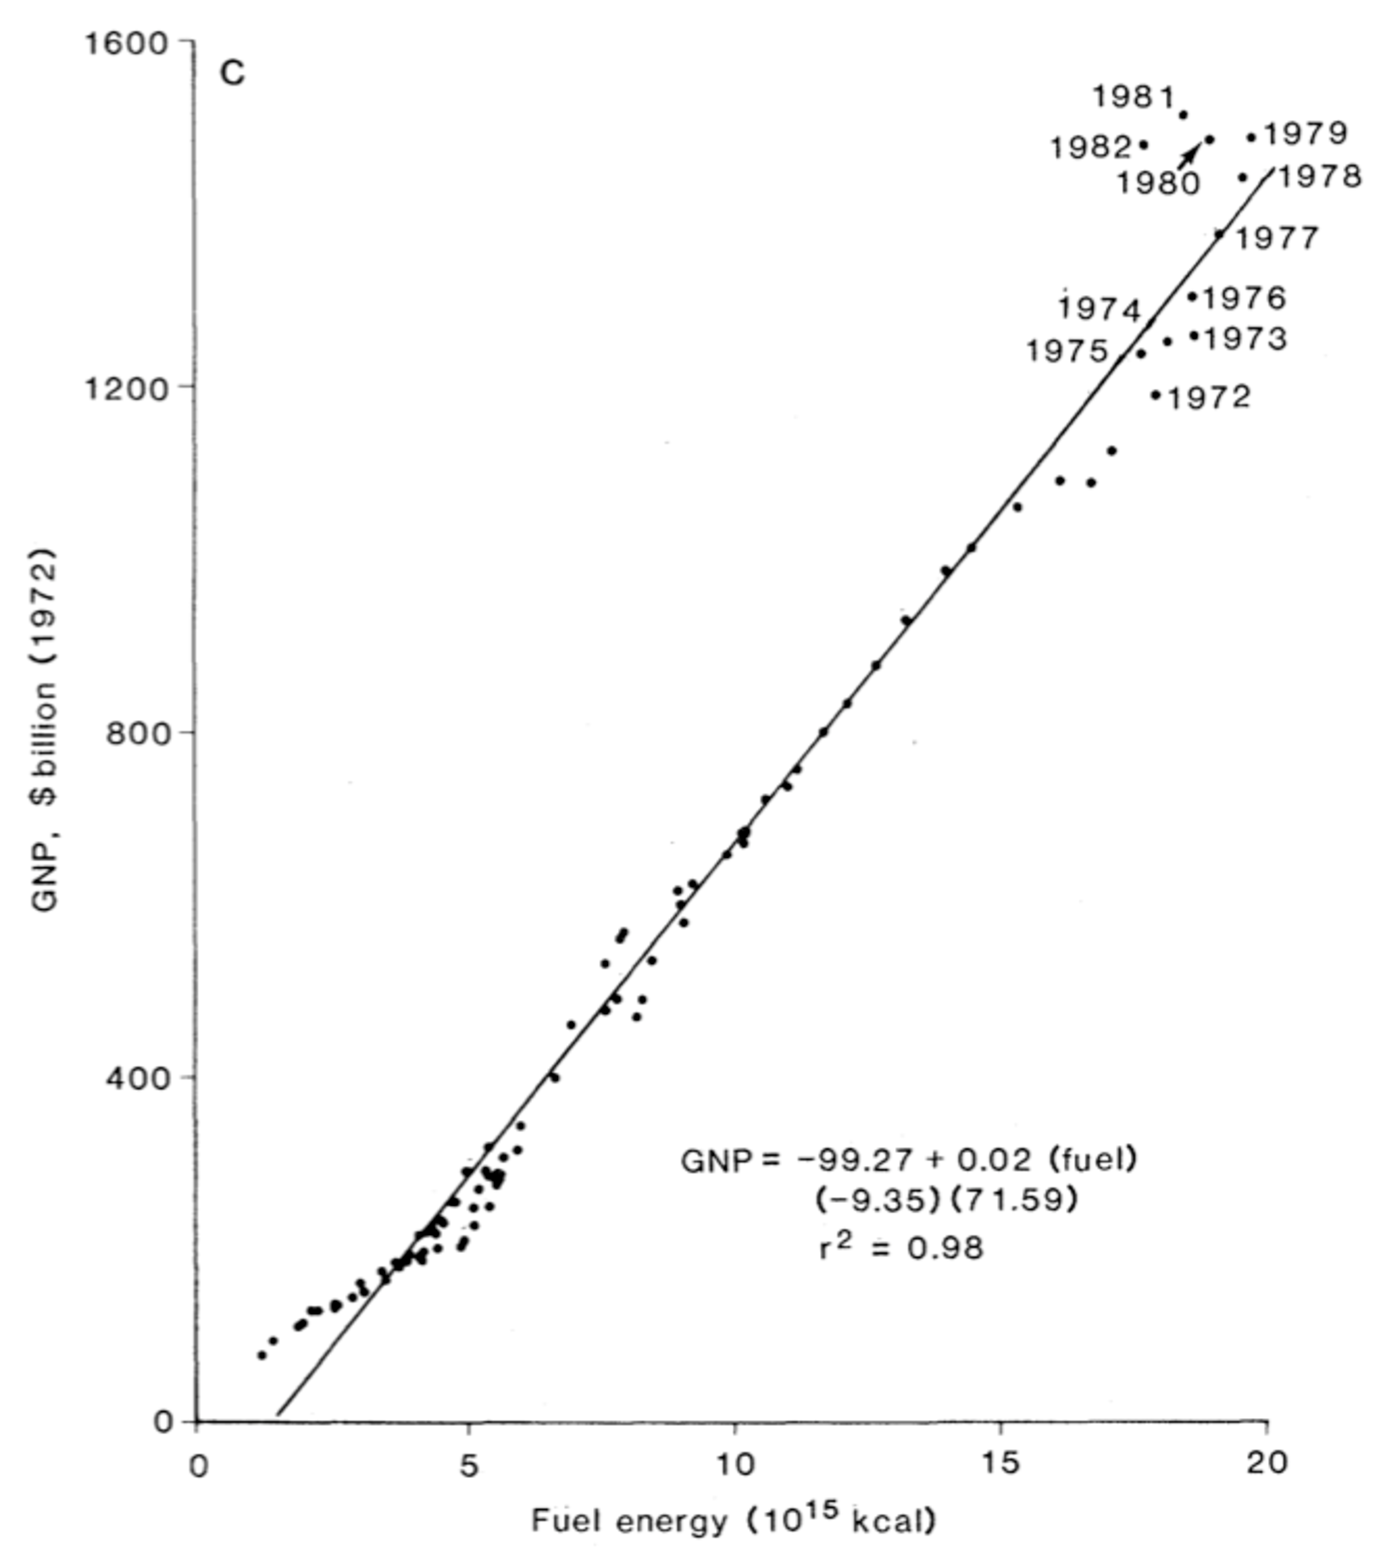
\includegraphics[width=\linewidth]{Part_0/Chapter_Introduction/images/Cleveland1984.pdf}
\caption[Energy and economic activity]{The famous graph from Cleveland, et.\ al.\
\cite{Cleveland:1984aa} showing the strong correlation 
between energy consumption and economic activity in the US from 1890 to 1982.
**** \copyright~\emph{Somebody. Used by permission.} ****}
% Permission to use this graph has been requested from Science. 
% See Copyright Permissions folder.
\label{fig:Cleveland1984}
\end{figure}

Because of the high correlation between energy consumption and economic activity,
it stands to reason that energy shortage relative to demand will hinder economic activity.
Of course, there are degrees of shortage. 
In extreme cases, and in the absence of price controls,
goods become hard to find and prices spike
as observed in the US during 1970s oil crisis.
(See Figure~\ref{fig:gas_shortage}.)

\begin{figure}[!ht]
\centering\
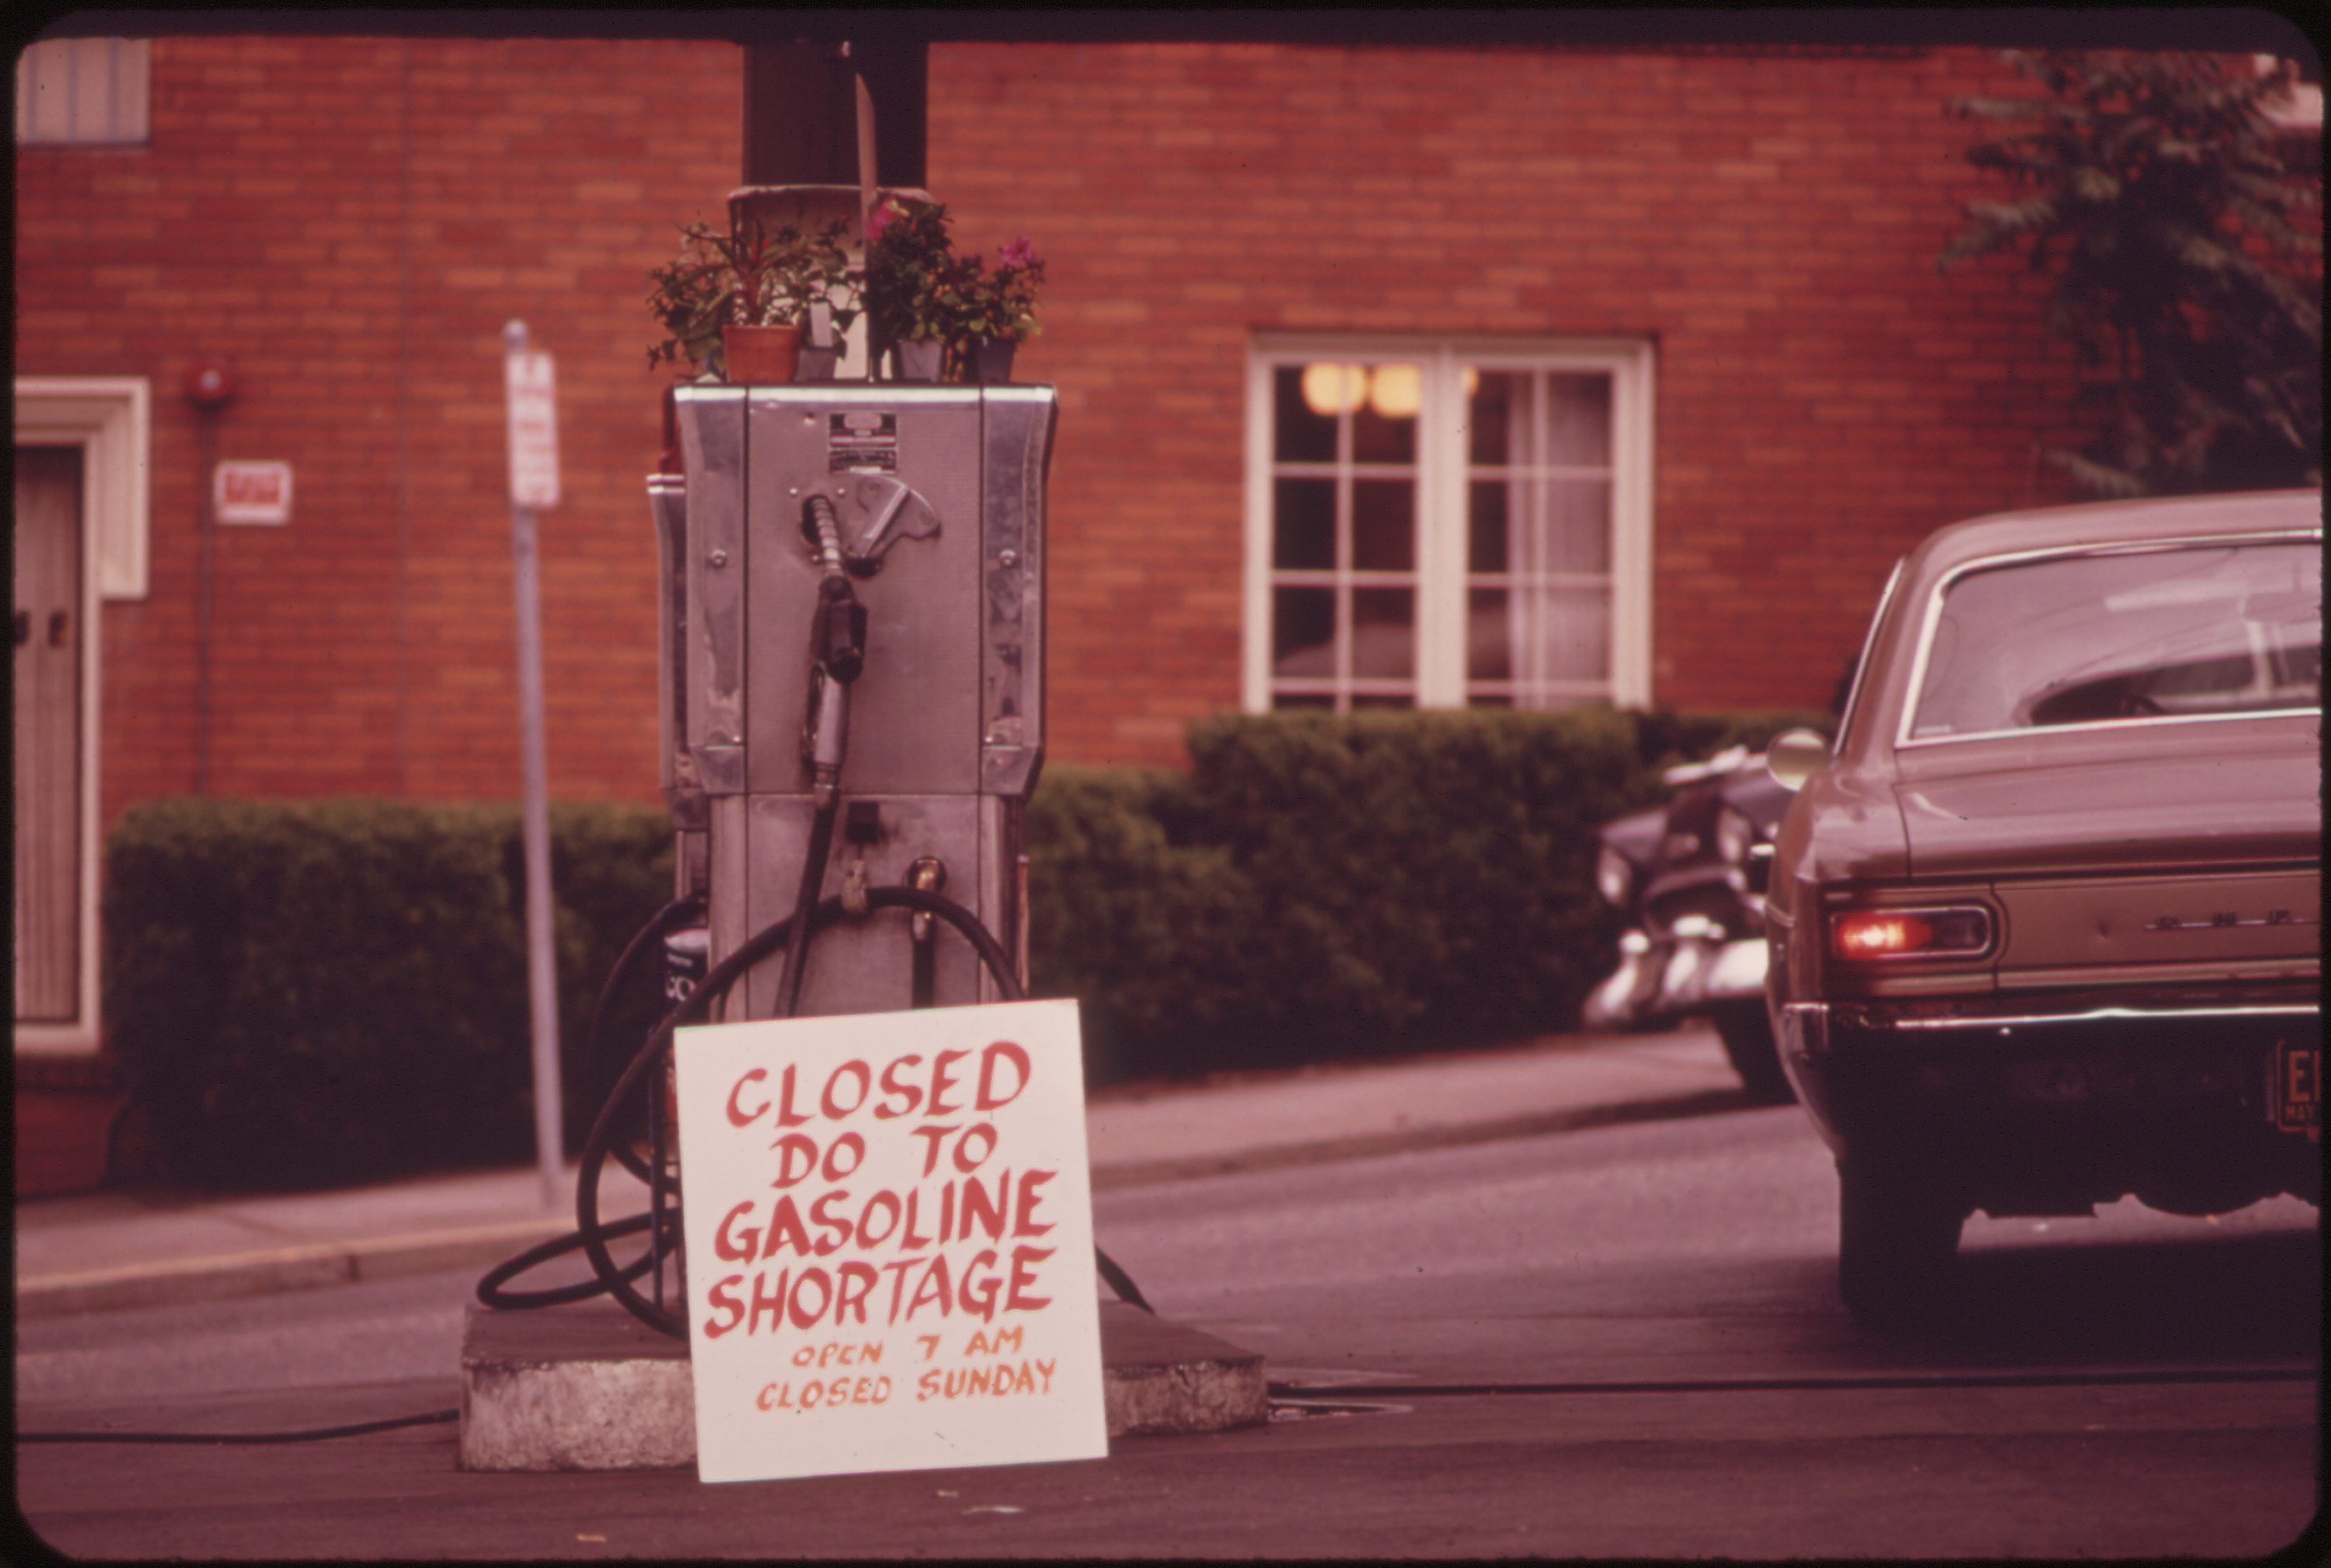
\includegraphics[width=\linewidth]{Part_0/Chapter_Introduction/images/gas_shortage_1973.jpg}
\caption[Gasoline shortage]{Gasoline shortages in 1973.\cite{Falconer:1973aa}}
% \url{http://arcweb.archives.gov/arc/action/ExternalIdSearch?id=548053}
% \url{https://www.flickr.com/photos/usnationalarchives/4272321708/in/set-72157623204210352/}}
\label{fig:gas_shortage}
\end{figure}

In mild cases,
shortage of any good relative to demand leads to rising prices,
even when goods remain available.
For example,
Figure~\ref{fig:oils_prices_and_production} shows oil prices (line) and 
worldwide oil production (vertical bars) 
before, during, and after the great recession. 
Demand for oil increased steadily in the early 2000s
due to worldwide economic growth, 
and production mostly kept pace through early 2005.
However, demand continued to increase while 
production flat-lined from early 2005 through late 2007, 
leading to a steep price increase.
From late 2007 through the end of 2008, 
the small amount of remaining reserve oil production was brought online,
but it was too little, too late.
Prices spiked above \$130/barrel in mid-2007. 
The great recession reduced demand slightly (by about 2 Mb/day)
and the price collapsed to about \$40/barrel.
Thereafter, demand and price rose to their previous levels 
as the world pulled out of the great recession.
In the years since 2008, oil production has risen slightly past the previous record highs
as additional production capacity has come online.

\begin{figure}[!ht]
\centering\
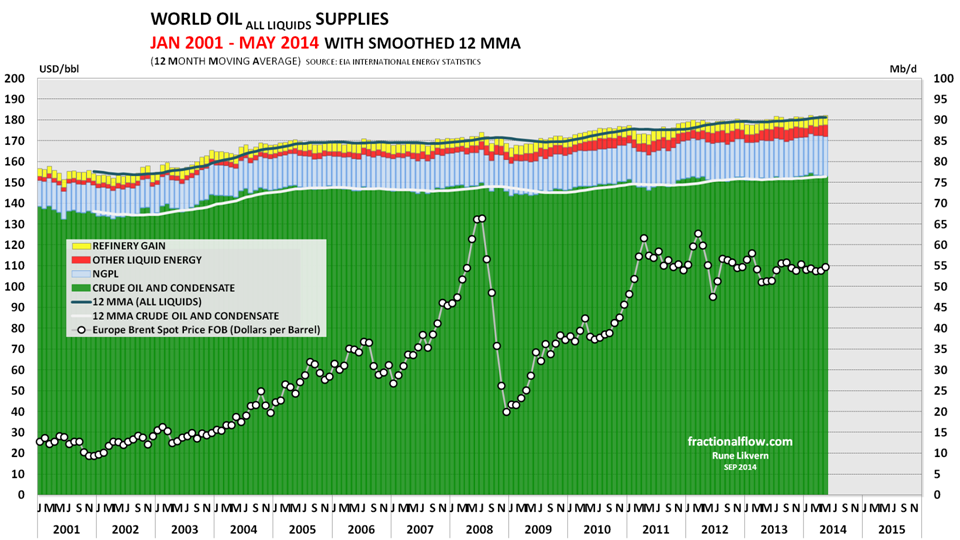
\includegraphics[width=\linewidth]{Part_0/Chapter_Introduction/images/WORLD_ALL_LIQUIDS_MAY_2014.png}
\caption[Oil prices and production)]{Oil prices~(left axis, data points) and production~(right axis, vertical bars). 
\copyright~\emph{Rune Likvern, {\scriptsize \emph{\url{http://www.fractionalflow.com}}}. Used by permission.}}
% Rune Likvern supplied and granted permission to use this graphic
% with attribution.
\label{fig:oils_prices_and_production}
\end{figure}

In both cases (1970s and 2000s), 
significant slowing of economic activity (recessions)
followed the oil shortages and prices spikes.
These were not isolated cases.
Hamilton noted that 
10 of the 11 US postwar recessions 
involved the same pattern.\cite[p.~45]{Hamilton:2013vc}
It is clear that 
there is a correlation between energy consumption and economic activity.

But, what are the dynamics that cause economic slowdowns 
to follow energy price spikes?
When prices rise faster than the cost of production, 
the profit motive should, according to economic theory, induce 
new firms to enter the market and
established firms to increase production.
However, the timing of supply and demand events is crucial.
If firms can't or don't increase production to meet demand, 
prices will remain elevated.
Even without increased production, falling demand will 
bring prices back to earth.

In terms of energy, and oil in particular, 
the \emph{rate} at which production can be increased 
is of the utmost importance, and
there are physical and technological limits. 
Consider this series of thought experiments:
We know that increasing the worldwide oil production rate by, say, 20\% 
involves
finding additional oil deposits, 
drilling additional wells, 
installing new pumps,
and expanding transport and delivery infrastructure worldwide.
In 1960, would it have been possible to achieve such an increase 
over a span of 5 years?
Yes. 
In fact, the worldwide oil production rate increased at a faster rate 
during the 1960s.
There was enough oil in the ground, 
and the economy could absorb the demand 
for additional steel, vehicles, energy, etc.\ required to emplace
the required infrastructure.
The impact on the financial system was minimal, 
because the cost of materials, equipment, labor, and energy
was spread out over a long-enough timeframe (in this thought experiment, 5 years). 
But, in 1960 could the oil production rate have been increased 
by 20\% in 3 months?
No.
There was enough oil in the ground,
but it would have been practically impossible to manufacture,
transport, and put into service all the necessary capital in such a short time.
Biophysical constraints limit the rate at which oil production can be increased.
What about 2 years?
Probably not.
It might have been physically possible, 
but the financial cost would have been too much to bear over such a short timeframe,
and the profit motive would be lost.

This thought experiment shows that time constraints,
layered upon physical and technological constraints, 
are the ties that bind the financial to the biophysical.
Put another way, time constraints are the point at which the economy 
becomes coupled to the biosphere.

In economic terms, biophysical constraints reduce the 
price elasticity of supply: 
the percent change in supply for a one percent change in price
during a given period of time.%
	\footnote{
	The mathematical definition of elasticity of supply ($E_s$) is
	\begin{equation*}
		E_s \equiv \frac{\frac{1}{Q}\frac{\partial Q}{\partial t}}
					{\frac{1}{P}\frac{\partial P}{\partial t}} \; ,
	\end{equation*}%
	where $Q$ is quantity of production, $P$ is price, and $t$ is time.
	}
Figure~\ref{fig:oils_prices_and_production} shows that 
a \emph{very large} percentage change in the price of oil was required to 
increase production by only a \emph{very small} percentage
in the 2005--2008 timeframe.
World oil production rose from 
78~million barrels per day to 86~million barrels per day,
an increase of only 10\%.\cite{EIA2014}
However, the inflation-adjusted price of oil increased 260\%,
from around \$35 to a peak of \$126 per barrel 
(in constant 2010 USD).
Thus, the supply of oil is nearly perfectly price inelastic, 
the short-run (2005-2008) price elasticity of the supply of oil 
is only 0.04.%
	\footnote{
	That is, a 1\% change in the oil price will generate
	only a 0.04\% increase in oil supply. 
	A price elasticity of 0.04 is extremely inelastic. 
	For comparison, agricultural output is also considered fairly price inelastic 
	in the short-run. 
	Pandey, et al.\ estimate the short-run (2-year) 
	price elasticity of supply of Australian agricultural output 
	to be around 0.30.\cite[p.~215]{pandey1982}
	}
Since 2010, the price of oil has remained over \$80 per barrel,
suggesting that production cannot increase quickly enough relative to demand
to bring prices back down to historical levels.
Persistently high prices for such an important commodity
suggest very real limits to production; 
supply is constrained relative to demand. 

In these circumstances, 
oil supply is said to be very \emph{inelastic} (unresponsive) to price.
The observed price inelasticity is caused by 
the biophysical limits to oil production discussed above.
Nothing, not even historically-high prices, can induce producers to 
increase the rate of supply in the short term (say, a 5-year time span), 
because it is physically impossible to do so.
In 2008, the world was running at full oil production capacity, 
but economies demanded more!
Because it was physically impossible to meet that demand,
prices spiked.

But, what caused the recession that followed?
Recently, a few authors have found that \emph{energy cost share},
the fraction of GDP spent on energy, 
is an explanatory variable for these dynamics.%
	\footnote{
	Mathematically, energy cost share ($f_E$) is defined as
	\begin{equation}
		f_E \equiv \frac{1}{GDP} \displaystyle\sum_i P_i Q_i \; ,
	\end{equation}
	where 
	the subscript $i$ indicates types of energy 
	(electricity, gasoline, natural gas, etc.),
	$P$ indicates the price of energy,
	$Q$ indicates the quantity of energy purchased within the economy, and
	$GDP$ is gross domestic product.
	}
To our knowledge, 
Bashmakov was the first to 
identify a long-term sustainable range for energy cost share
in mature economies.\cite{Bashmakov:2007ek} 
He also showed that developed economies 
can sustain high total energy cost share
for a short period of time 
(possibly 2--3 years) 
before recessionary pressures 
destroy energy demand,%
	\footnote{
	Note that ``destruction of energy demand'' 
	is accomplished through recession
	in the short run.
	}
stimulate energy efficiency,%
	\footnote{
	Like increasing oil production, 
	increasing energy efficiency also has 
	physical and technological limits.
	Improving energy efficiency is a medium- to long-term process. 
	}
reduce energy prices, 
and return total energy cost share to its long-term sustainable range.
On the other hand, reduction of total energy cost share below 
a lower bound provides economic stimulus, 
increases energy demand, 
provides upward pressure on energy prices, 
and returns energy cost share to its long-term sustainable range.
Bashmakov speculates that 
``energy affordability thresholds and behavioral constants'' 
are responsible for the stable range of energy cost share 
over many decades.\cite[p.~3585]{Bashmakov:2007ek} 
The long-term stable range for economy-wide energy cost share 
(which includes all forms of energy, including oil, natural gas, and electricity)
is 9--11\% for the OECD. 
For oil only, Murphy and Hall found that 
the oil cost share threshold that correlates with US recessions 
is about 5.5\%.\cite{Murphy:2011jh}

The picture emerging from this research shows that 
the cost share of energy in the economy
(and, perhaps more narrowly, oil cost share in the economy)
is an important factor in stimulating or restraining economic growth,
despite its small value (typically, less than 10\%).%
	\footnote{
	Embarking on an economic growth path
	appears to reduce the energy cost share in an economy from very high values
	(indicating that nearly all economic activity is focused on procuring energy)
	to small values that remain within a stable range.
	For example, Sweden's energy cost share has stabilized at 12\% since 1970,
	although it was nearly 100\% in 1800.\cite{Stern:2012ey}.
	}
It appears that the economy-biosphere system has 
a built-in feedback mechanism that 
enforces alignment between biophysical limits and the economy.

This may be somewhat surprising in light of mainstream economic theory, 
which ascribes economic importance 
based on financial cost share, 
not biophysical factors. 
Indeed, the cost share of energy in mature economies is low, 
and viewing energy as relatively unimportant is justified if
one's view of ``importance'' is limited to financial information only.
But, many have noted that the physical importance of energy to the economy 
far exceeds its cost share.\cite{Ayres:2013aa}
And, as discussed above, because the economy is coupled 
to the biophysical world through time constraints (as manifest 
by the low price elasticity of energy supply), 
the physical importance of energy far exceeds its financial importance.
Ironically, low energy cost share 
is precisely the condition that 
has allowed economies to be incredibly productive over the last century.

The connection between energy and the economy may be difficult to see, 
but, eventually, it becomes impossible to ignore.


%+++++++++ Stall related to non-renewable stocks ++++++++++
\subsection{Stalled growth is related to non-renewable stocks}
\label{sec:stall_non-renewable_stocks}
%+++++++++

Given the tight coupling between the biosphyical world and the economy,
especially regarding energy,
discussed in Section~\ref{sec:energy-economy_coupling} above,
it is prudent to consider the important economic role of
material and energy stocks in the biosphere.

The Best-First Principle~\cite{Cleveland:2008aa}
indicates that the economy will extract the easiest-to-obtain 
stocks of mineral and energy resources first.
``Best'' and ``easiest'' can be assessed in several ways, 
but physical factors that make a resource ``best'' or ``easiest to extract'' 
eventually manifest as lower cost.
For example, inexpensive-to-obtain West Texas crude oil was extracted
before expensive-to-obtain offshore oil. 
Surface deposits of gold and diamonds are exhausted before subsurface
veins and kimberlite pipes are exploited.
High-purity mineral deposits are exploited before low-purity deposits.
As a result, it becomes more ``difficult'' to continually increase
extraction rates as time proceeds.
To continue with our energy example,
historical oil production trends reflect these realities.
Through time, the annual rate of increase of oil production
has declined from 7.8\%/year to 0.7\%/year.
(See Figure~\ref{fig:oil_production}.)

\begin{figure}[!ht]
\centering\
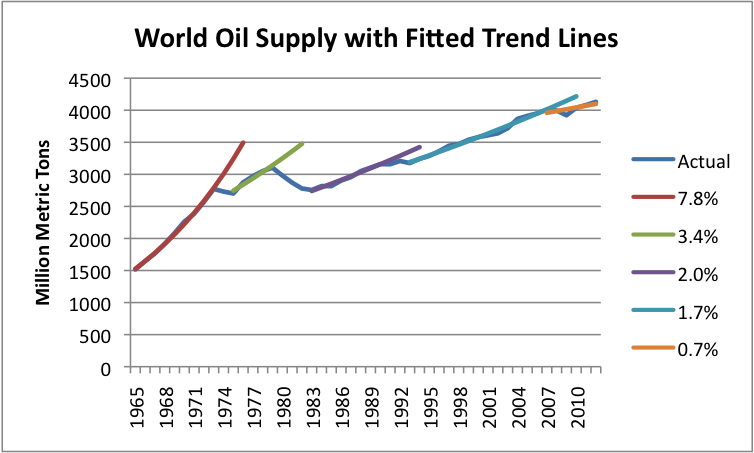
\includegraphics[width=\linewidth]{Part_0/Chapter_Introduction/images/growth-in-world-oil-supply.png}
\caption[World Oil Supply]{Slowing growth in world oil supply.\cite[Figure~3]{Tverberg:2013aa}
\copyright~\emph{Gail Tverberg, {\scriptsize \emph{\url{http://www.ourfiniteworld.com}}}. Used by permission.}}
% Permission to use this graph was granted by Gail Tverberg free of charge.
% See Copyright Permissions folder for the email that she sent.
\label{fig:oil_production}
\end{figure}

It is important to realize that it takes energy to make energy available to society.
Oil production requires energy for the ongoing
operation of pumps, 
transportation of crude to the refinery,
refinement of crude to useable petroleum products, and 
transportation of refined products to consumers and firms.
In addition, it takes energy to manufacture the wells, pumps, 
tankers, pipelines, and
refineries used in oil production and distribution.
Furthermore, it takes energy to use energy. 
The economy uses energy to manufacture the machines (vehicles, mostly)
that consume refined oil products.

Application of the Best-First Principle to the energy production process 
indicates that it will take more energy 
to make energy available to society as non-renewable 
energy resources in the biosphere are depleted.
The metric that measures the energy impacts of the Best-First Principle is 
Energy Return on Investment ($EROI_{soc}$), 
the ratio of energy provided to society 
by the energy consumed in making it available.%
	\footnote{
	Energy return on investment ($EROI_{soc}$) at the societal level is defined as 
	%
	\begin{equation}
		EROI_{soc} \equiv \frac{\dot{E}_a}{\dot{E}_c} \; ,
	\end{equation}
	%
	where $\dot{E}_a$ is the rate of energy made available to society in MJ/year
	and $\dot{E}_c$ is the rate of energy consumed in the energy production process in MJ/year.
	Note that this definition of $EROI_{soc}$ is flow based.
	Other definitions of $EROI$ are accounted over the full lifetime of a project,
	e.g., comparing the lifetime electricity generation of a wind turbine
	to the energy required in its 
	manufacture (including extraction of raw materials),
	installation,
	operation and,
	decommission.
	}
As energy resources in the biosphere are depleted, 
the Best-First Principle entails that
$EROI_{soc}$ will decline.
Indeed it has.
Turning again to our oil example, $EROI_{soc}$ for production of US oil has declined 
from a value of 23 in the 1950s
to 10 in 2007.\cite[Fig.~2]{Guilford:2011ci}
$EROI_{soc}$ for production of oil worldwide has declined 
from a value of 35 in 1999
to 18 in 2006.\cite[Fig.~1]{Gagnon:2009fc}.
In other words, it takes about twice as much energy today
than in years past
to make a barrel of oil available to society.

Furthermore, declining $EROI_{soc}$ for oil has economic impacts.
Both Heun and de~Wit~\cite{Heun:2012ek} and King and Hall~\cite{King:2011go}
show that declining $EROI_{soc}$ correlates with higher prices for oil, 
because declining $EROI_{soc}$ provides upward pressure on 
production costs, and therefore, prices
as time proceeds.

All other things being equal, the Best-First Principle
indicates that the additional physical ``effort'' required to extract
increasingly-marginal resources will lead to decreased extraction rates.
In the race against the Best-First Principle,
technological advances can bring about higher extraction rates, 
despite the additional physical ``effort'' required. 
The early 19$^{\mathrm{th}}$ Century economist David Ricardo applied this 
principle to the theory of land rents. 
As population increases, 
the demand for food will increase. 
Because arable land is not reproducible, 
less-productive land will be utilized for crops. 
This leads to increasing profits accruing to owners of the best land.

In the energy markets, recent increases in unconventional oil production
(from tar sands and shale)
have been made possible by new extraction and refining technologies.
But most unconventional oil production is accompanied 
by the same or lower $EROI_{soc}$
compared to conventional crude oil production. 
% See http://theenergycollective.com/robertrapier/314966/cost-production-and-energy-return-oil-sands
% for Robert Rapier's estimate of EROI for oil sands.
% Also see Cutler Cleveland on Oil Shale:
% http://www.westernresourceadvocates.org/land/pdf/oseroireport.pdf
Furthermore, today's unconventional oil is more expensive to produce
than the crude of yesteryear.
Consequently, oil prices must remain high for 
unconventional production to remain financially feasible into the foreseeable future. 
Unfortunately, Section~\ref{sec:energy-economy_coupling} showed that
high energy prices can lead to high energy cost share in the economy
and recessionary pressure.

The fact that shortages of crude oil provide incentives for 
technological advancements that bring unconventional production online 
appears, at first glace, to be a good thing.
However, energy substitutions are beneficial to society 
in the long run only when the $EROI_{soc}$ of the substitute
is equal to or higher than the original.
Thus, the benefits of unconventional oils are modest, at best, when the
high financial and energy costs of production are considered.

That said, transitions to new sources of energy will be a feature 
of the economy in the age of resource depletion.
But, there is evidence of limits to energy substitution 
at the macroeconomic level.
Pelli, in a study of 21 countries 
found that clean%
	\footnote{
	Nuclear, 
	conventional hydroelectric power, wood and waste biomass, 
	geothermal, solar/photovoltaic, and wind
	}
and dirty%
	\footnote{
	Coal, 
	petroleum, natural gas, and other gasses
	}
inputs to electricity production
are complementary (as opposed to substitutable).\cite{Pelli:2012wv}
His conclusion is dire:
%
\begin{quote}
	On the one hand, according to the model, 
	if we keep producing electricity using dirty inputs, 
	we head toward an environmental disaster. 
	On the other hand, looking at the empirical results, 
	it seems impossible to stop producing electricity with polluting resources. 
	The policy implication of this paper thus, 
	seems to be that we need more important subsidies to research, 
	as fast as possible, 
	and high carbon taxes combined with a complete halt 
	of the growth rate of the production of electricity. 
	In this way, according to the model, 
	we may be able to avoid an environmental disaster.\cite[p.~25]{Pelli:2012wv}
\end{quote}

In a meta-analysis of 15 papers that studied 
the economic evidence for macro-substitutability
among factors of production (materials, capital, labor, and energy), 
de Wit et.\ al.~\cite{de-Wit:2013aa} found that the elasticity of substitution was 
below unity for all combinations of factors of production.
Furthermore, they argue that, 
%
\begin{quote}
	[because all of the] results show elasticity of substitution below unity, 
	none of the factor inputs are perfectly substitutable, and 
	all tend toward complementarity in varying degrees. 
	Such results suggest that transitions 
	from one production or consumption structure to another 
	can be disruptive and that the transitions 
	need to be modeled dynamically to the extent possible.\cite[p.~8]{de-Wit:2013aa}
\end{quote}

The challenges of energy substitutions are highlighted
when examining the financial situation of oil producers.
Figure~\ref{fig:oil_company_free_cash_flow} 
shows that despite the recent increase in oil production rate
and continued high prices, 
the free cash flow%
	\footnote{
	Free cash flow is defined as the cash produced by a firm's operations
	less the cost of expanding its asset base. 
	Free cash flow is different from profit,
	and is thought to be a more-reliable indicator of the ability of a firm
	to produce profit.
	}
of independent oil producers is negative.
This situation implies that capital investments are unproductive to date.
It remains to be seen how independent producers 
can continue advancing the oil production rate (which implies capital investment)
while their free cash flow is negative.
One possible cure is higher oil prices.
But, again, we saw 
in Section~\ref{sec:energy-economy_coupling}
that high energy cost share 
provides recessionary pressure.

\begin{figure}[!ht]
\centering\
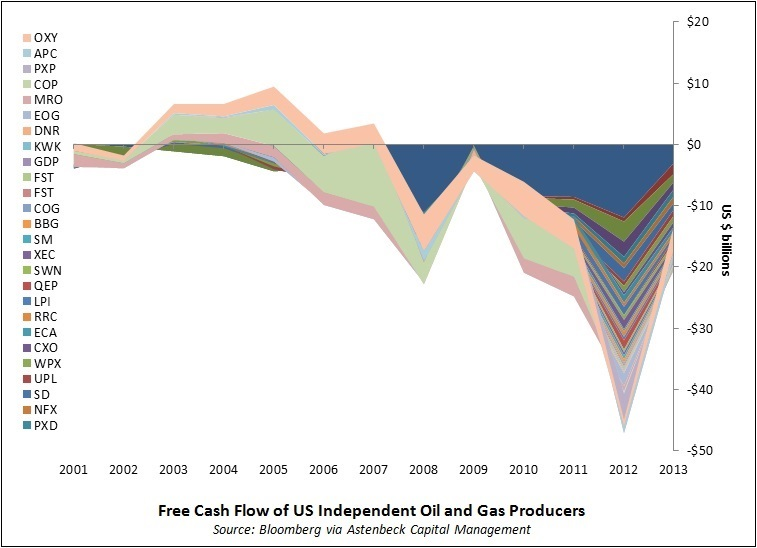
\includegraphics[width=\linewidth]{Part_0/Chapter_Introduction/images/Cash-Flow.jpg}
\caption[Oil company free cash flow]{Oil company free cash flow.\cite{Kopits:2014aa}
**** \copyright~\emph{Somebody. Used by permission.} ****}
% \url{http://blogs.platts.com/2014/07/30/peak-oil-forecasts/}
% Permission to use this figure has been requested from Steve Kopits, 
% even though he may not own the copyright. 
\label{fig:oil_company_free_cash_flow}
\end{figure}

All of this comes about simply because it is 
more physically ``difficult,'' and, as a consequence, 
more financially expensive
to extract oil today than it was just a few decades ago.
It is more difficult to obtain oil today because we have depleted
the stocks of easy-to-obtain crude oil from the biosphere.
And, the remaining stocks are either lower quality (e.g., shale)
or further away (e.g., deeper offshore).

We contend that similar dynamics will apply to 
any non-renewable material (e.g. copper, fish, soil, timber) 
or energy stock (natural gas, hydro dam sites)
in the biosphere
for which substitution is difficult.
Using oil as our example, we observe that 
stocks of natural capital, especially energy resources,
have significant economic implications.
Both the declining \emph{quantity} and 
the diminishing \emph{quality} of remaining non-renewable biosphere stocks 
are contributing to the slowdown of growth in mature economies
discussed in the opening to this chapter.

Stocks of another sort also play a role 
in the slowdown of growth experienced by mature economies,
because they  are important drivers of material and energy consumption.
In the next section, we turn our attention 
away from the biosphere 
toward the economy and its stock of capital.


%+++++++++ Stall related to capital stock ++++++++++
\subsection{Stalled growth is related to capital stock}
\label{sec:stall_capital_stock}
%+++++++++

Capital is extremely valuable and, in most cases, essential to production processes:
machines reduce per-unit costs of production;
buildings provide space to work and protection for capital;
roads provide networks for vehicular transport 
of raw materials, finished goods, and capital itself; and
computers enhance the efficiency of workers and enable technological breakththroughs.
There are several types of capital flows
to and from its stock in the economy.
We use the term ``emplacement'' to denote a flow of capital into
the economy, for example when a new machine is put into service,
when a new building is constructed, or
when a new road is opened.
``Depreciation'' is normal wear-and-tear experienced by capital, 
a type of outflow of capital from the economy.
Financial depreciation involves the write-off of a percentage 
of the value of capital.
Physical depreciation involves wear and tear of parts within or sections of the capital.
Financial depreciation usually occurs faster than physical depreciation.
``Maintenance'' is servicing of capital to overcome the effects of physical depreciation.
``Disposal'' is the physical outflow of capital from the economy to the biosphere
upon removal from service.
Capital ``formation'' is the rate of net
addition to capital stock in the economy,
the difference between inflows and outflows
during a time interval.
Traditionally, stocks and flows of capital are measured by currency units, 
\$ and \$/year, respectively.
However, we argue later (Section~\ref{sec:Implications_for_IO})
that a physical basis for capital accounting is also warranted.

It is important to note that it takes materials and energy
to manufacture and emplace capital at its point of use.
Furthermore, once emplaced,
capital consumes energy to process raw materials 
into intermediate and finished products
and for its maintenance.
The energy required to manufacture and emplace capital
(including all upstream processes)
is called \emph{embodied} energy.
In addition to capital, energy is embodied in all manufactured materials and
products.%
	\footnote{
	See Chapter~\ref{chap:embodied_energy} for more details
	on embodied energy.
	}
The ratio of energy embodied in products to their price 
is the energy \emph{intensity} of output ($\varepsilon$, 
in units of J/\$).%
	\footnote{
	See Chapter~\ref{chap:intensity} for more details 
	on energy intensity.
	}
Both embodied energy and energy intensity are key metrics 
for understanding the economy.
To first approximation, energy embodied in capital provides an estimate of the 
energy needed for replacement.
The distribution of energy intensity
across products and sectors
provides a picture of energy demands caused by consumption.

Most capital (especially machines) is considerably more expensive
than the individual products it makes.
So, it takes significant financial resources (relative to sales) 
to purchase and emplace capital.
Capital is so beneficial (i.e., productive in the economic sense), 
that firms pursue and obtain debt financing to cover large capital expenses.
In the case of public goods like roads, bridges, and utilities,
governments pursue debt financing via municipal bonds.
The long-term financial obligations associated with capital financing 
mean that the capital is expected to be in service
for at least the repayment period of the debt,
usually much longer.

The long-term commitment to capital and production means that 
emplacement of capital is a bond, a claim on future
raw material and energy \emph{consumption}.
And, it is an assurance of raw material and energy \emph{extraction} 
from the biosphere for many years to come.
Furthermore, extant productive capital stock can't be fed just any material or energy;
capital is designed to work with only certain types of materials and energy.
An auto body panel stamping machine is designed to form steel, perhaps even a specific 
grade or alloy of steel;
feeding plastic won't do.
The machine likely runs on electricity; 
feeding gasoline won't do.

Thus, the stock of capital in the economy 
is an important driver of not only 
the rate but also  
the type of
material and energy flows from the biosphere.
The emplacement of productive capital
``locks in'' demand for specific types of materials and energy 
into the forseeable future.
As such, long-term commitments associated with emplaced capital
provide limits to the rate at which society can effect
transitions to different raw materials and energy sources.
Again, we observe tight coupling between the economy and the biosphere!

Given the discussion in Section~\ref{sec:stall_non-renewable_stocks}
regarding the economic dynamics 
of biophysical limits to raw material and energy extraction,
we see that expansion of an economy's capital stock may increase GDP
in the short run, 
but it also ``locks in'' 
future material and energy demands 
from the biosphere.
These ``locked in'' demands bring the economy closer 
to the biophysical extraction limits 
that will eventually lead to economic slowdown.

\begin{svgraybox}
	Paradoxically, and contrasting with mainstream policy prescriptions,
	expansion of the stock of capital in the economy 
	can contribute to the ultimate slowdown of economic growth.
\end{svgraybox}


%%%%%%%%%% Consumption-driven policies are unsustainable %%%%%%%%%%
\section{Consumption-driven solutions are unsustainable}
\label{sec:consumption_unsustainable}
%%%%%%%%%%

In Section~\ref{sec:stall_capital_stock} above, 
we noted that today's consumption-enhancing policies have the side-effect of
increasing many material and energy flow rates into the economy.
Thus, today's policies also
hasten the day when we reach binding biophysical constraints
due to resource depletion. 
Unfortunately, biophysical limits 
are not included in the mainstream economic thinking and modeling
that informs today's policy decisions.%
	\footnote{
	More on the problematic nature of this oversight
	can be found in Sections~\ref{sec:three_epochs} and~\ref{sec:age_of_resource_depletion}.
	}
Three factors, in combination, are vitally important 
but nearly-always ignored: 
(1) the economy is tightly coupled to the biosphere, 
(2) there are physical and technological limits 
	to the rate at which materials and energy can be extracted 
	from the biosphere, and 
(3) today's emplacement of manufactured capital locks in
	tomorrow's material and energy demands 
	for both operation and maintenance of that capital.
Set against the backdrop of Section~\ref{sec:exogenous_factors},
we see that consumption-enhancing policies are ineffective,
because of the biophysical limits that ultimately constrain the scale of the economy. 

In short, the economic analyses that support 
consumption-driven policies are incomplete.
Consumption-driven economic growth is ultimately unsustainable.

Adoption of consumption-enhancing policies when society is already encountering
resource depletion constraints
will result in see-saw economic performance. 
In fact, we may have already entered a regime of boom-bust economic dynamics,
because of a binding constraint for oil extraction rate
as discussed in Section~\ref{sec:exogenous_factors}.
In the face of see-saw dynamics,
it is difficult to make wise and insightful long-term investment or policy decisions,
because you're perpetually recovering from the most-recent bust.

In the age of resource depletion, 
we need to move beyond GDP.
These dynamics should cause us to measure and report
the material and energy demands that products and capital stock 
make upon the biosphere.
We should know these factors 
in \emph{physical} as well as financial terms,
for constraints of the physical world 
lead to problems in the economy.
These data should be available routinely from a centralized location.

This is the end of an era.
In mature economies, consumption-enhancing 
economic policies can no longer guarantee 
growth of living standards and well-being.
But, the mainstream is blind to what should be done instead. 


%%%%%%%%%% Change is needed %%%%%%%%%%
\section{Change is needed!}
\label{sec:change_needed}
%%%%%%%%%%

The fact that we (as a society) do not include exogenous, biophysical factors 
in economic decision-making indicates that
we do not fully understand how the real economy operates.
Society is ignorant of the role that natural and manufactured%
	\footnote{
	Manufactured capital presupposes the existance of 
	significant levels of human and social capital.
	}
capital together play in both sustaining today's economy and 
constraining future economic prospects and choices.
At present, markets are virtually the only tool at our disposal
to help us understand the characteristics of the real economy.
What benefits do markets provide?
Markets are, at least in economic theory, extremely efficient allocators of resources,
provided that all relevant information is available to market participants.
Mainstream economic theory holds that prices are the mechanism by which signals
of value are communicated to sellers and buyers:
sellers receive information about how goods are valued by consumers, and
buyers receive information about the cost of materials accrued by producers.

In the age of resource depletion, 
are price signals sufficient to indicate shortages, 
especially of important and difficult-to-substitute resources?
It appears that some signals are getting through.
Heun and de Wit
showed that scarcity (as indicated by low $EROI_{soc}$)
correlates with higher oil prices.\cite{Heun:2012ek}
And, higher prices spur efficiency improvements.\cite{Vlasic:2013aa}

However, the market's price mechanism may not be enough.
We showed in Section~\ref{sec:energy-economy_coupling}
that the physical importance 
of scarce and difficult-to-substitute resources (e.g., oil) 
far exceeds cost share in the economy,
suggesting that prices alone cannot provide comprehensive
signals of importance to producers and consumers.
Consequently, producers and consumers participate 
in the market with incomplete information.
This is a serious problem, 
because the allocative efficiency of markets 
is predicated upon
correct and complete information being available to market participants.

Furthermore, a good must be owned before 
it can be sold.
Thus, prices cannot be set and market value cannot be determined
for goods that are not considered ``property,'' 
such as clean water, clean air, and other ``ecosystem services.''
In addition, today's markets are simply incapable of deciding
important issues such as the optimal scale (size) of the economy
relative to the biosphere. (See Section~\ref{sec:metabolic_scale}.)

In the age of resource depletion, the allocative efficiency of markets is attractive.
Indeed, life would be better if the markets could shift supply and demand away from
binding biophysical constraints when they are encountered. 
But, lack of information
in today's markets leads us to argue that they are not up to the task. 
Today's markets are a poor choice for allocative decisions 
about scarce and difficult-to-substitute resources (such as oil)
or non-property goods (such as clean air, clean water, and other ecosystem services).

What additional information would be helpful?
We contend that detailed information about energy, embodied energy, and energy intensity
would be a good place to start.
We, as a society, routinely account and publish energy flow rates only.%
	 \footnote{
	 Energy consumption rates are routinely published by the 
	 US Energy Information Agency (EIA) and the 
	 International Energy Agency (IEA).
	 }
We do not, however, routinely update energy \emph{intensity}%
	\footnote{
	Estimates of energy intensity are not included in systems of national accounts.
	And, such work is rarely undertaken by academics.\citep{Bullard1975, EIOLCA2014} 
	}
estimates ($\varepsilon$)
and, therefore, 
we have little idea of where energy is embodied 
in our capital stock and 
in the products we consume.
Furthermore, when energy intensity ($\varepsilon$) of products is estimated, 
it does not account for the energy embodied in our stock of capital
and is therefore in error.%
	\footnote{
	See Section~\ref{sec:Implications_for_IO} for our suggested remedy.
	}
	
We suggest that all of this information 
(economic, material, and energy indicators) 
should be collated by a single agency and
reported from a single location.
Doing so will provide convenience and consistency and
indicate the interconnectness of the economy and the biosphere
to both policymakers and researchers.

We understand that these suggested changes will be both 
revolutionary in scope and
challenging to implement politically.
Therefore, we would do well to be sure of our direction.
We would do well to put ourselves on rigorous and firm theoretical grounding
\emph{before} proceeding toward implementation. 
The role of this book is to provide just that:
a rigorous theoretical framework
for a better system of national accounts,
one that goes beyond GDP and
one that is relevant to the age of resource depletion.

Until these crucial pieces of information are routinely available 
in a centralized location within a rigorous theoretical framework, 
society will be unable to properly frame and conceptualize 
the ``problem'' of ``stalling'' growth. 
Until this information is available to markets,
investment, consumption, and policy decisions cannot
lead to socially optimal outcomes.



\bibliographystyle{unsrt}
\bibliography{../../Metabolic}


% Always give a unique label
% and use \ref{<label>} for cross-references
% and \cite{<label>} for bibliographic references
% use \sectionmark{}
% to alter or adjust the section heading in the running head
%% Instead of simply listing headings of different levels we recommend to let every heading be followed by at least a short passage of text. Furtheron please use the \LaTeX\ automatism for all your cross-references and citations.

%% Please note that the first line of text that follows a heading is not indented, whereas the first lines of all sequent paragraphs are.

%% Use the standard \verb|equation| environment to typeset your equations, e.g.
%
%% \begin{equation}
%% a \times b = c\;,
%% \end{equation}
%
%% however, for multiline equations we recommend to use the \verb|eqnarray|
%% environment\footnote{In physics texts please activate the class option \texttt{vecphys} to depict your vectors in \textbf{\itshape boldface-italic} type - as is customary for a wide range of physical jects.}.
%% \begin{eqnarray}
%% a \times b = c \nonumber\\
%% \vec{a} \cdot \vec{b}=\vec{c}
%% \label{eq:01}
%% \end{eqnarray}

%% \section{section Heading}
%% \label{sec:2}
%% Instead of simply listing headings of different levels we recommend to let every heading be followed by at least a short passage of text. Furtheron please use the \LaTeX\ automatism for all your cross-references\index{cross-references} and citations\index{citations} as has already been described in Sect.~\ref{sec:2}.

%% \begin{quotation}
%% Please do not use quotation marks when quoting texts! Simply use the \verb|quotation| environment -- it will automatically render Springer's preferred layout.
%% \end{quotation}


%% \section{section Heading}
%% Instead of simply listing headings of different levels we recommend to let every heading be followed by at least a short passage of text. Furtheron please use the \LaTeX\ automatism for all your cross-references and citations as has already been described in Sect.~\ref{sec:2}, see also Fig.~\ref{fig:1}\footnote{If you copy text passages, figures, or tables from other works, you must obtain \textit{permission} from the copyright holder (usually the original publisher). Please enclose the signed permission with the manucript. The sources\index{permission to print} must be acknowledged either in the captions, as footnotes or in a separate section of the book.}

%% Please note that the first line of text that follows a heading is not indented, whereas the first lines of all sequent paragraphs are.

% For figures use
%
%% \begin{figure}[b]
%% \sidecaption
% Use the relevant command for your figure-insertion program
% to insert the figure file.
% For example, with the option graphics use
%% \includegraphics[scale=.65]{figure}
%
% If not, use
%\picplace{5cm}{2cm} % Give the correct figure height and width in cm
%
%% \caption{If the width of the figure is less than 7.8 cm use the \texttt{sidecapion} command to flush the caption on the left side of the page. If the figure is positioned at the top of the page, align the sidecaption with the top of the figure -- to achieve this you simply need to use the optional argument \texttt{[t]} with the \texttt{sidecaption} command}
%% \label{fig:1}       % Give a unique label
%% \end{figure}


%% \paragraph{Paragraph Heading} %
%% Instead of simply listing headings of different levels we recommend to let every heading be followed by at least a short passage of text. Furtheron please use the \LaTeX\ automatism for all your cross-references and citations as has already been described in Sect.~\ref{sec:2}.

%% Please note that the first line of text that follows a heading is not indented, whereas the first lines of all sequent paragraphs are.

%% For typesetting numbered lists we recommend to use the \verb|enumerate| environment -- it will automatically render Springer's preferred layout.

%% \begin{enumerate}
%% \item{Livelihood and survival mobility are oftentimes coutcomes of uneven socioeconomic development.}
%% \begin{enumerate}
%% \item{Livelihood and survival mobility are oftentimes coutcomes of uneven socioeconomic development.}
%% \item{Livelihood and survival mobility are oftentimes coutcomes of uneven socioeconomic development.}
%% \end{enumerate}
%% \item{Livelihood and survival mobility are oftentimes coutcomes of uneven socioeconomic development.}
%% \end{enumerate}


%% \paragraph{paragraph Heading} In order to avoid simply listing headings of different levels we recommend to let every heading be followed by at least a short passage of text. Use the \LaTeX\ automatism for all your cross-references and citations as has already been described in Sect.~\ref{sec:2}, see also Fig.~\ref{fig:2}.

%% Please note that the first line of text that follows a heading is not indented, whereas the first lines of all sequent paragraphs are.

%% For unnumbered list we recommend to use the \verb|itemize| environment -- it will automatically render Springer's preferred layout.

%% \begin{itemize}
%% \item{Livelihood and survival mobility are oftentimes coutcomes of uneven socioeconomic development, cf. Table~\ref{tab:1}.}
%% \begin{itemize}
%% \item{Livelihood and survival mobility are oftentimes coutcomes of uneven socioeconomic development.}
%% \item{Livelihood and survival mobility are oftentimes coutcomes of uneven socioeconomic development.}
%% \end{itemize}
%% \item{Livelihood and survival mobility are oftentimes coutcomes of uneven socioeconomic development.}
%% \end{itemize}

%% \begin{figure}[t]
%% \sidecaption[t]
% Use the relevant command for your figure-insertion program
% to insert the figure file.
% For example, with the option graphics use
%% \includegraphics[scale=.65]{figure}
%
% If not, use
%\picplace{5cm}{2cm} % Give the correct figure height and width in cm
%
%% \caption{Please write your figure caption here}
%% \label{fig:2}       % Give a unique label
%% \end{figure}

%% \runinhead{Run-in Heading Boldface Version} Use the \LaTeX\ automatism for all your cross-references and citations as has already been described in Sect.~\ref{sec:2}.

%% \runinhead{Run-in Heading Italic Version} Use the \LaTeX\ automatism for all your cross-refer\-ences and citations as has already been described in Sect.~\ref{sec:2}\index{paragraph}.
% Use the \index{} command to code your index words
%
% For tables use
%
%% \begin{table}
%% \caption{Please write your table caption here}
%% \label{tab:1}       % Give a unique label
%
% For LaTeX tables use
%
%% \begin{tabular}{p{2cm}p{2.4cm}p{2cm}p{4.9cm}}
%% \hline\noalign{\smallskip}
%% Classes & class & Length & Action Mechanism  \\
%% \noalign{\smallskip}\svhline\noalign{\smallskip}
%% Translation & mRNA$^a$  & 22 (19--25) & Translation repression, mRNA cleavage\\
%% Translation & mRNA cleavage & 21 & mRNA cleavage\\
%% Translation & mRNA  & 21--22 & mRNA cleavage\\
%%Translation & mRNA  & 24--26 & Histone and DNA Modification\\
%%\noalign{\smallskip}\hline\noalign{\smallskip}
%%\end{tabular}
%%$^a$ Table foot note (with superscript)
%%\end{table}
%
%% \section{Section Heading}
%%\label{sec:3}
% Always give a unique label
% and use \ref{<label>} for cross-references
% and \cite{<label>} for bibliographic references
% use \sectionmark{}
% to alter or adjust the section heading in the running head
%% Instead of simply listing headings of different levels we recommend to let every heading be followed by at least a short passage of text. Furtheron please use the \LaTeX\ automatism for all your cross-references and citations as has already been described in Sect.~\ref{sec:2}.

%% Please note that the first line of text that follows a heading is not indented, whereas the first lines of all sequent paragraphs are.

%%If you want to list definitions or the like we recommend to use the Springer-enhanced \verb|description| environment -- it will automatically render Springer's preferred layout.

%%\begin{description}[Type 1]
%%\item[Type 1]{That addresses central themes pertainng to migration, health, and disease. In Sect.~\ref{sec:1}, Wilson discusses the role of human migration in infectious disease distributions and patterns.}
%%\item[Type 2]{That addresses central themes pertainng to migration, health, and disease. In Sect.~\ref{sec:2}, Wilson discusses the role of human migration in infectious disease distributions and patterns.}
%%\end{description}

%%\section{section Heading} %
%% In order to avoid simply listing headings of different levels we recommend to let every heading be followed by at least a short passage of text. Use the \LaTeX\ automatism for all your cross-references and citations citations as has already been described in Sect.~\ref{sec:2}.

%% Please note that the first line of text that follows a heading is not indented, whereas the first lines of all sequent paragraphs are.

%% \begin{svgraybox}
%% If you want to emphasize complete paragraphs of texts we recommend to use the newly defined Springer class option \verb|graybox| and the newly defined environment \verb|svgraybox|. This will produce a 15 percent screened box 'behind' your text.

%% If you want to emphasize complete paragraphs of texts we recommend to use the newly defined Springer class option and environment \verb|svgraybox|. This will produce a 15 percent screened box 'behind' your text.
%% \end{svgraybox}


%% \section{section Heading}
%%Instead of simply listing headings of different levels we recommend to let every heading be followed by at least a short passage of text. Furtheron please use the \LaTeX\ automatism for all your cross-references and citations as has already been described in Sect.~\ref{sec:2}.

%% Please note that the first line of text that follows a heading is not indented, whereas the first lines of all sequent paragraphs are.

%% \begin{theorem}
%% Theorem text goes here.
%% \end{theorem}
%
% or
%
%% \begin{definition}
%% Definition text goes here.
%% \end{definition}

%% \begin{proof}
%\smartqed
%% Proof text goes here.
%% \qed
%% \end{proof}

%%\paragraph{Paragraph Heading} %
%% Instead of simply listing headings of different levels we recommend to let every heading be followed by at least a short passage of text. Furtheron please use the \LaTeX\ automatism for all your cross-references and citations as has already been described in Sect.~\ref{sec:2}.

%% Note that the first line of text that follows a heading is not indented, whereas the first lines of all subsequent paragraphs are.
%
% For built-in environments use
%
%%\begin{theorem}
%%Theorem text goes here.
%%\end{theorem}
%
%%\begin{definition}
%%Definition text goes here.
%%\end{definition}
%
%%\begin{proof}
%%\smartqed
%% Proof text goes here.
%%\qed
%%\end{proof}
%
%% \begin{acknowledgement}
%% If you want to include acknowledgments of assistance and the like at the end of an individual chapter please use the \verb|acknowledgement| environment -- it will automatically render Springer's preferred layout.
%% \end{acknowledgement}
%
%% \section*{Appendix}
%% \addcontentsline{toc}{section}{Appendix}
%
%% When placed at the end of a chapter or contribution (as opposed to at the end of the book), the numbering of tables, figures, and equations in the appendix section continues on from that in the main text. Hence please \textit{do not} use the \verb|appendix| command when writing an appendix at the end of your chapter or contribution. If there is only one the appendix is designated ``Appendix'', or ``Appendix 1'', or ``Appendix 2'', etc. if there is more than one.

%% \begin{equation}
%% a \times b = c
%% \end{equation}
% Problems or Exercises should be sorted chapterwise
%% \section*{Problems}
%% \addcontentsline{toc}{section}{Problems}
%
% Use the following environment.
% Don't forget to label each problem;
% the label is needed for the solutions' environment
%% \begin{prob}
%% \label{prob1}
%% A given problem or Excercise is described here. The
%% problem is described here. The problem is described here.
%% \end{prob}

%% \begin{prob}
%% \label{prob2}
%% \textbf{Problem Heading}\\
%% (a) The first part of the problem is described here.\\
%% (b) The second part of the problem is described here.
%% \end{prob}


